

\documentclass[DIV=calc, paper=a4, fontsize=10.5pt]{scrartcl}
\usepackage{makeidx}
\usepackage{graphicx}
\usepackage{flushend}
\usepackage{amssymb}


\usepackage{lmodern}
\usepackage[left=1.5cm,right=1.5cm,top=2.5cm,bottom=2cm]{geometry}
\usepackage{float}		
\bibliographystyle{plain} 
\pagestyle{plain} 
\pagenumbering{arabic}
\usepackage{fancyhdr} 	
\usepackage[T1]{fontenc}
\usepackage[utf8]{inputenc}
\usepackage[spanish]{babel}
\usepackage[spanish,es-tabla]{babel}
\usepackage{hyperref}
\usepackage{graphicx}
\usepackage{siunitx}
\usepackage{lipsum}
\usepackage[protrusion=true,expansion=true]{microtype}
\usepackage{amsmath,amsfonts,amsthm}
\usepackage[svgnames]{xcolor}
\usepackage[svgnames]{xcolor}
\usepackage{booktabs}
\usepackage{fix-cm}
\usepackage{multicol}
\usepackage{url}
\usepackage{cancel}
\usepackage{subfig}
\bibliographystyle{unsrt}

\newenvironment{Figura}
  {\par\medskip\noindent\minipage{\linewidth}}
  {\endminipage\par\medskip}

\usepackage{sectsty}
\allsectionsfont{\usefont{OT1}{phv}{b}{n}}
\usepackage{fancyhdr}
\spanishdecimal{.}
\pagestyle{fancy}
\usepackage{lastpage}
\lhead{}
\chead{}
\rhead{}
\lfoot{}
\cfoot{}
\rfoot{\footnotesize Page \thepage\ of \pageref{LastPage}}
\renewcommand{\headrulewidth}{0.0pt}
\renewcommand{\footrulewidth}{0.4pt}
\usepackage{lettrine}
\newcommand{\initial}[1]{\lettrine[lines=3,lhang=0.3,nindent=0em]{
\color{DarkGoldenrod}{\textsf{#1}}}{}}
\usepackage{titling}
\newcommand{\HorRule}{\color{DarkGoldenrod} \rule{\linewidth}{1pt}}
\pretitle{\vspace{-120pt} \begin{flushleft} \HorRule \fontsize{22}{35} \usefont{OT1}{phv}{b}{n} 
\color{DarkRed} \selectfont}
\title{Práctica 10. \\ %Aquí va el nombre de la práctica 
Interferencia y Difracción} %Numero de la práctica 
\posttitle{\par
\end{flushleft}
\vskip 0.5em}
\preauthor{\begin{flushleft}\large \lineskip 0.5em \usefont{OT1}{phv}{b}{sl} \color{DarkRed}}
\author{Angel Yair García Pérez \\
Misael Iván Macías Márquez\\
Teodora Irene Ortíz Cruz\\
\small{teodora625@ciencias.unam.mx}\\}
\postauthor{\footnotesize \usefont{OT1}{phv}{m}{sl} \color{Black}
\vspace*{0.1cm} 
Facultad de Ciencias, UNAM
\par\end{flushleft}\HorRule}
\date{20 de Mayo de 2022\\Semestre 2022-2}
\begin{document}
\maketitle
\definecolor{carmine}{rgb}{0.59, 0.0, 0.09}
\begin{abstract}

  \textcolor{carmine}{Resumen:} Por medio de un arreglo experimental basado en el experimento Young, se midieron las posiciones de los mínimos del patrón de interferencia con respecto al centro. Se obtuvo que la primer distancia entre rendijas era de $(0.0805\hspace{0.1cm}\pm\hspace{0.1cm}0.0002)\hspace{0.1cm}\text{ mm}$ con una discrepancia de $52.5\hspace{0.1cm}>\hspace{0.1cm}2$ y  $\Delta_{\%}=2.4\%$, para la segunda se tiene un valor de $(0.1020\hspace{0.1cm}\pm\hspace{0.1cm}0.0001)\hspace{0.1cm}\text{ mm}$ con discrepancia de $6.66\hspace{0.1cm}>\hspace{0.1cm}2$ y una $\Delta_{\%}=0.29\%$, para la tercer rendija el valor fue de $(0.1480\hspace{0.1cm}\pm\hspace{0.1cm}0.0001)\hspace{0.1cm}\text{ mm}$  discrepancia de $4\hspace{0.1cm}>\hspace{0.1cm}2$ y una $\Delta_{\%}=0.33\%$, para la última rendija se obtuvo un valor de $(0.1580\hspace{0.1cm}\pm\hspace{0.1cm}0.0001)\hspace{0.1cm}\text{ mm}$ con discrepancia de $4\hspace{0.1cm}>\hspace{0.1cm}2$ y una  $\Delta_{\%}=0.31\%$. Se obtuvo una longitud de onda del láser verde de  $\lambda_{\text{verde}} = (521 \pm 6) \text{ nm}$ con una discrepancia de $0.16\hspace{0.1cm}<\hspace{0.1cm}2$ y una $\Delta_{\%}=86.8\%$. Por otro lado, con rendijas sencillas se obtuvo que el ancho de la primer rendija era de $(0.2120\hspace{0.1cm}\pm\hspace{0.1cm}0.0001)\hspace{0.1cm}\text{ mm}$ con una discrepancia de $120\hspace{0.1cm}>\hspace{0.1cm}2$ y una i $\Delta_{\%}=0.04\%$, para la segunda rendija se obtuvo un valor de  $(0.1720\hspace{0.1cm}\pm\hspace{0.1cm}0.0001)\hspace{0.1cm}\text{ mm }$con una discrepancia de $70\hspace{0.1cm}>\hspace{0.1cm}2$ y una  $\Delta_{\%}=0.05\%$, para la última rendija se obtuvo $(0.2050\hspace{0.1cm}\pm\hspace{0.1cm}0.0001)\hspace{0.1cm}\text{ mm }$con una discrepancia de $50\hspace{0.1cm}>\hspace{0.1cm}2$ y una  $\Delta_{\%}=0.04\%$. Se obtuvo una longitud de onda     $\lambda_{\text{verde}} = (555 \pm 3) \text{ nm}$ con una discrepancia $11.6\hspace{0.1cm}<\hspace{0.1cm}2$ y una $\Delta_{\%}=0.54\%$. Se considera que la primer longitud de onda obtenida es un resultado satisfactorio.
\end{abstract}
\section*{\textcolor{carmine}{Introducción.}}
El objetivo de este trabajo es caracterizar los tamaños de rendijas de  interferencia y difracción, así como encontrar la longitud de onda de algún láser a partir de medidas de los patrones de interferencia \cite{Manual}. La importancia de está practica radica en familiarizarse con el fenómeno de difracción el cual ha jugado un papel importante dentro de la investigación científica para analizar algunas estructuras como el ADN \cite{Manual}. Se espera que se cumpla el modelo teórico propuesto en la literatura \cite{book} y partiendo de los valores de la hoja de datos del láser verde se espera encontrar que el valor de la longitud de onda para el láser verde sea de $520\text{ nm}\pm10\text{ nm}$ y con el láser rojo se espera encontrar que los valores de las rendijas son de $a_1 = 0.07 \text{ mm}$, $a_2= 0.10 \text{ mm}$, $a_3 = 0.15 \text{ mm}$ y $a_4 = 0.16 \text{ mm}$ para las dobles rendijas y $b_1 = 0.2 \text{ mm}$, $b_2 = 0.165 \text{ mm}$ y $0.210 \text{ mm}$ para las rendijas simples.
\subsection*{\textcolor{carmine}{Interferencia}}
La interferencia óptica equivale a la interacción de dos o más ondas de luz que producen una irradiancia resultante que se desvía de la suma de las irradiancias componentes. Hay varias formas de producir este fenómeno, sin embargo el experimento de Young es una de las formas más importantes de producirla debido a las implicaciones físicas que tiene\cite{book}. 
El arreglo experimental se basaba en una fuente de luz que atravesaba por dos rendijas, creando luz coherente que posteriormente cruzaría por dos rendijas como se muestra en la Figura 1. 
Si se considera que la doble rendija esta a una distancia L y que la separación entre las rendijas es a se puede formar un triangulo se tiene que 
\begin{equation*}
    \Delta=s_{2}-s_{1}=a\sin{\theta}
\end{equation*}
Utilizando las ecuaciones de irradiancia\cite{Manual} se obtiene que las posición de las franjas cuando hay interferencia constructiva es 
\begin{equation*}
    y_{max}=\frac{mL\lambda}{a}
\end{equation*}
Y si es destructiva las posición de las franjas oscuras es
\begin{equation}
    y_{min}=\frac{L\lambda}{a}\left(m\pm\frac{1}{2}\right)
\end{equation}
\begin{figure}[H]
    \centering
    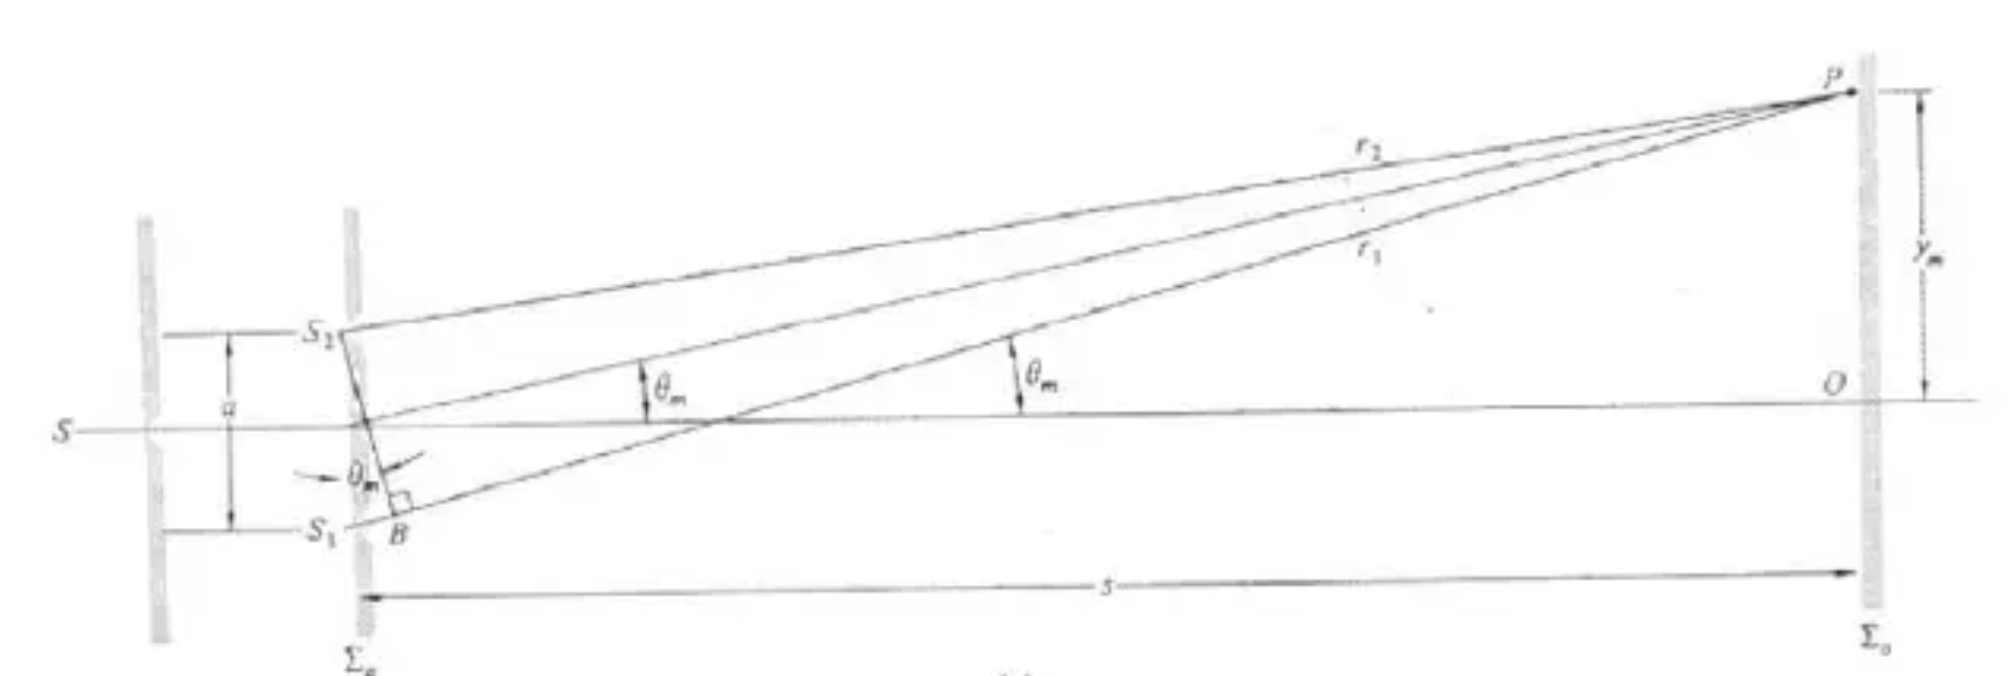
\includegraphics[width=9cm]{Captura de Pantalla 2022-05-31 a la(s) 16.29.23.png}
    \caption{Diagrama de la geometría del experimento de la doble rendija para calcular la funciones que arrojan los mínimos y máximos.\cite{book}}
    \label{fig:my_label}
\end{figure}
\subsection*{\textcolor{carmine}{Difracción}}
Las aperturas del experimento de Young son anchas de tal forma en que no se puede considerar que son puntuales por lo que suele producir un efecto de interferencia y ocurre incluso cuando hay solo una apertura y se le llama difracción. Para estudiarlo consideremos que una luz monocromática atraviesa una rendija 
como se muestra en la Figura 1. La condición de interferencia destructiva en difracción es 
\begin{equation*}
    m\lambda=b\sin{\theta}
\end{equation*}
y los mínimos se pueden encontrar usando la aproximación de ángulo pequeño y la ecuación de irradiancia para este caso \cite{Manual}
\begin{equation}
     y_{min}=\frac{mL\lambda}{b}
\end{equation}
\begin{figure}[H]
    \centering
    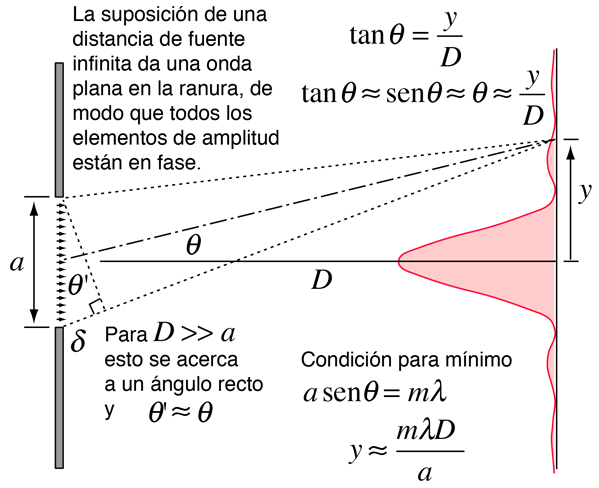
\includegraphics[width=6cm]{fraungeo.png}
    \caption{Geometría del arreglo experimental experimental para difracción. Se puede observar también la aproximación de ángulo pequeño mencionada.\cite{pagina}}
    \label{fig:my_label}
\end{figure}

\section*{\textcolor{carmine}{Desarrollo Experimental.}}
\textbf{\textcolor{carmine}{Interferencia de Young.}}\\
Para esta parte se colocó el láser sobre la mesa óptica y frente a el las rendijas doble de distinta separación, como se muestra en la Figura 3. Luego se encendió el láser y se apunto hacia alguna de las rendijas de tal manera en que  el patrón de interferencia se viera nítido en la pared, en esa zona de la pared se colocó una hoja de papel.\\ Para poder medir la distancia de la rendija a la pantalla se utilizó una cinta métrica y a las medidas se les asocio una incertidumbre de apreciación $\sigma_{ap}=\pm\hspace{0.1cm}0.05\hspace{0.1cm}cm$. Con un vernier se midió las posición de los mínimos, es decir las franjas negras, con respecto del centro. La incertidumbre de apreciación asociada a estas medidas fue de $\sigma_{ap}=\pm\hspace{0.1cm}0.005\hspace{0.1cm}mm$. Luego se repitió el mismo procedimiento para 3 rendijas distintas a la misma distancia de la pantalla. Posterior a ello, se cambió la distancia de la pantalla y se repitió el experimento para las mismas 4 rendijas anteriores. Por último se cambió el láser rojo por un láser verde y se repitió el experimento asumiendo que lo que se conocía era el valor de separación de las rendijas y no la longitud de onda.
\begin{figure}[H]
 \centering
  \subfloat[Arreglo experimental para observar la interferencia de Young.]{
   \label{f:gato}
    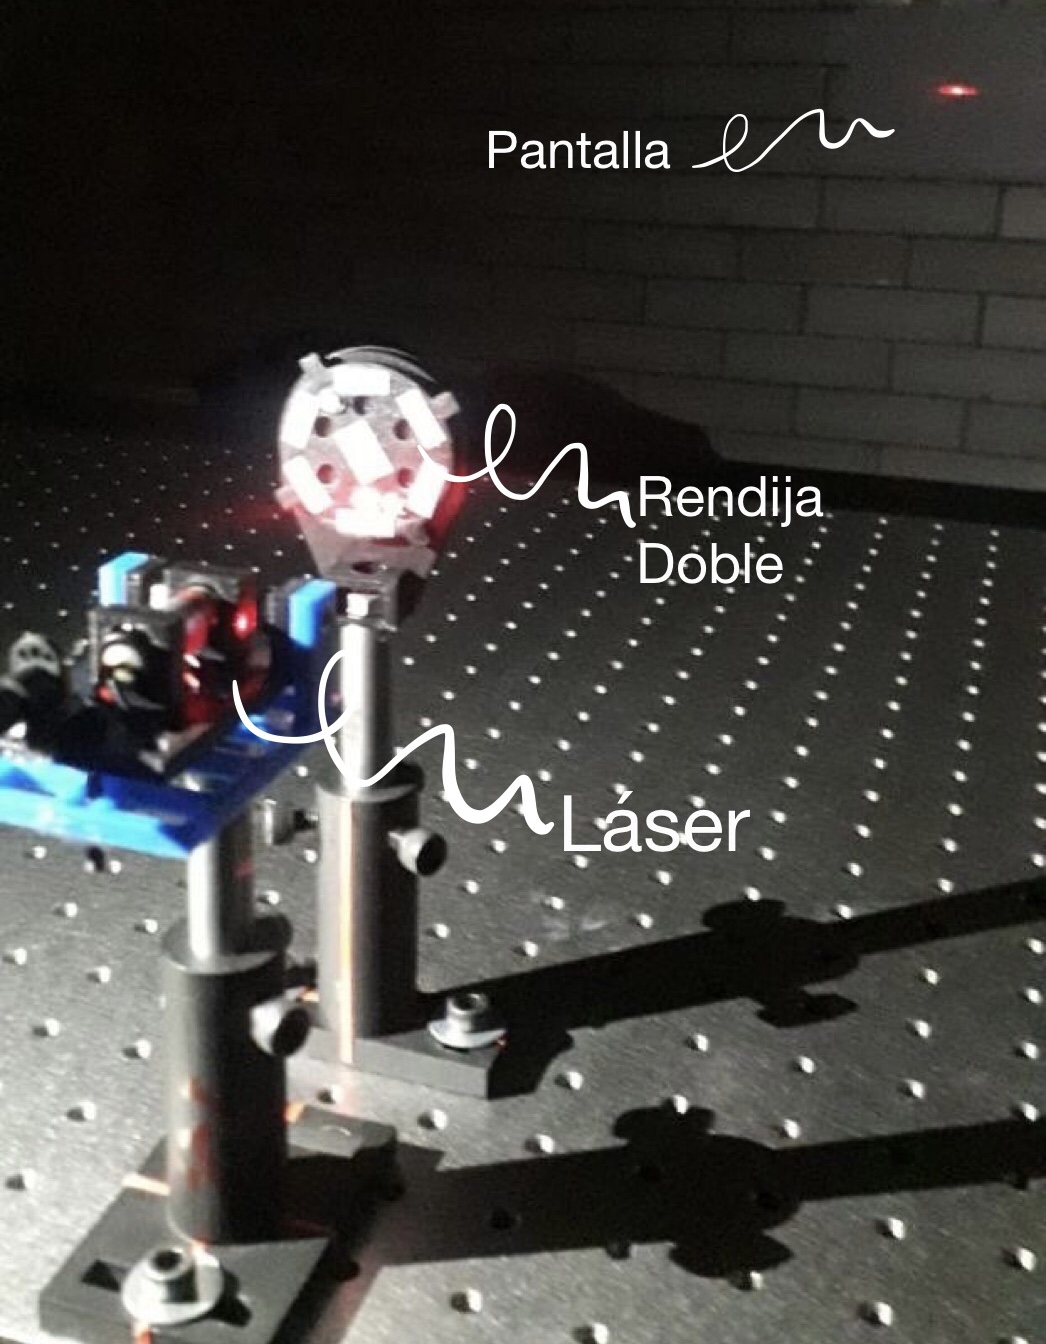
\includegraphics[width=0.25\textwidth]{Desarrollo experimental/C53E10CE-A9B7-43E2-B926-F3958E41358C.jpeg}}
  \subfloat[Franjas de interferencia vistas en el experimento]{
   \label{f:tigre}
    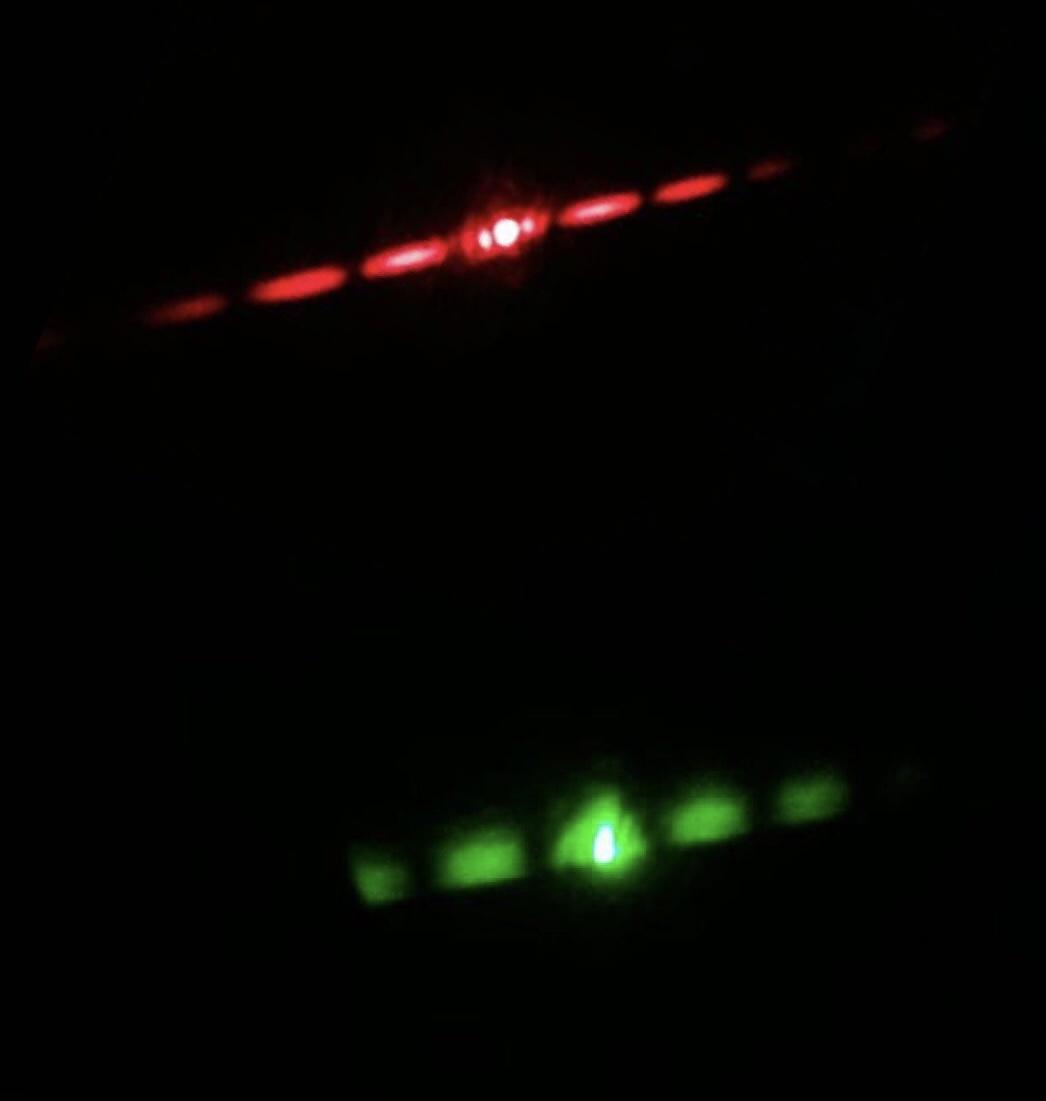
\includegraphics[width=0.3\textwidth]{Desarrollo experimental/AE6866AF-766A-41B5-88D2-71F11B5CE8F7.jpeg}}
 \caption{\textbf{Experimento de Young.} En la figura 3(a) se observa el arreglo experimental utilizado para observar lo patrones de interferencia de una doble rendija. En la figura 3(b) se observan los patrones de interferencia vistos para el láser rojo y verde. }
 \label{f:animales}
\end{figure}

\textbf{\textcolor{carmine}{Difracción.}}\\
Se colocó el láser rojo  sobre la mesa óptica y frente a el se puso una rendija sencilla como se muestra en la Figura 4(a). Luego se encendió el láser y se apunto hacia la rendija, de tal manera en que  el patrón de interferencia, como el que se muestra en la figura 4(b), se viera nítido en la pared, en esa zona de la pared se colocó una hoja de papel.\\Para poder medir la distancia de la rendija a la pantalla se utilizó una cinta métrica y a las medidas se les asoció una incertidumbre de apreciación $\sigma_{ap}=\pm\hspace{0.1cm}0.05\hspace{0.1cm}cm$. Luego con una pluma de punto muy fino, se marco el centro del patrón de interferencia y se dibujaron las franjas, luego con un vernier se midió la distancia de las franjas oscuras  marcadas en la pantalla con respecto del centro dibujado. Este último método se implemento para hacer más cómoda la medición de franjas. A las distancias medidas con el vernier se les asoció una incertidumbre de apreciación $\sigma_{ap}=\pm\hspace{0.1cm}0.005\hspace{0.1cm}mm$. 
Este procedimiento se repitió para otras 3 rendijas sencillas sencillas distintas
a la misma distancia de la pantalla. Posterior a ello, se cambió la distancia de la pantalla y se repitió el experimento para las mismas 4 rendijas anteriores.
Por último se cambió el láser rojo por un láser verde y se repitió el experimento asumiendo que lo que se conocía era el valor de separación de las rendijas y no la longitud de onda.
\begin{figure}[H]
 \centering
  \subfloat[Arreglo experimental para observar la difracción.]{
   \label{f:gato}
    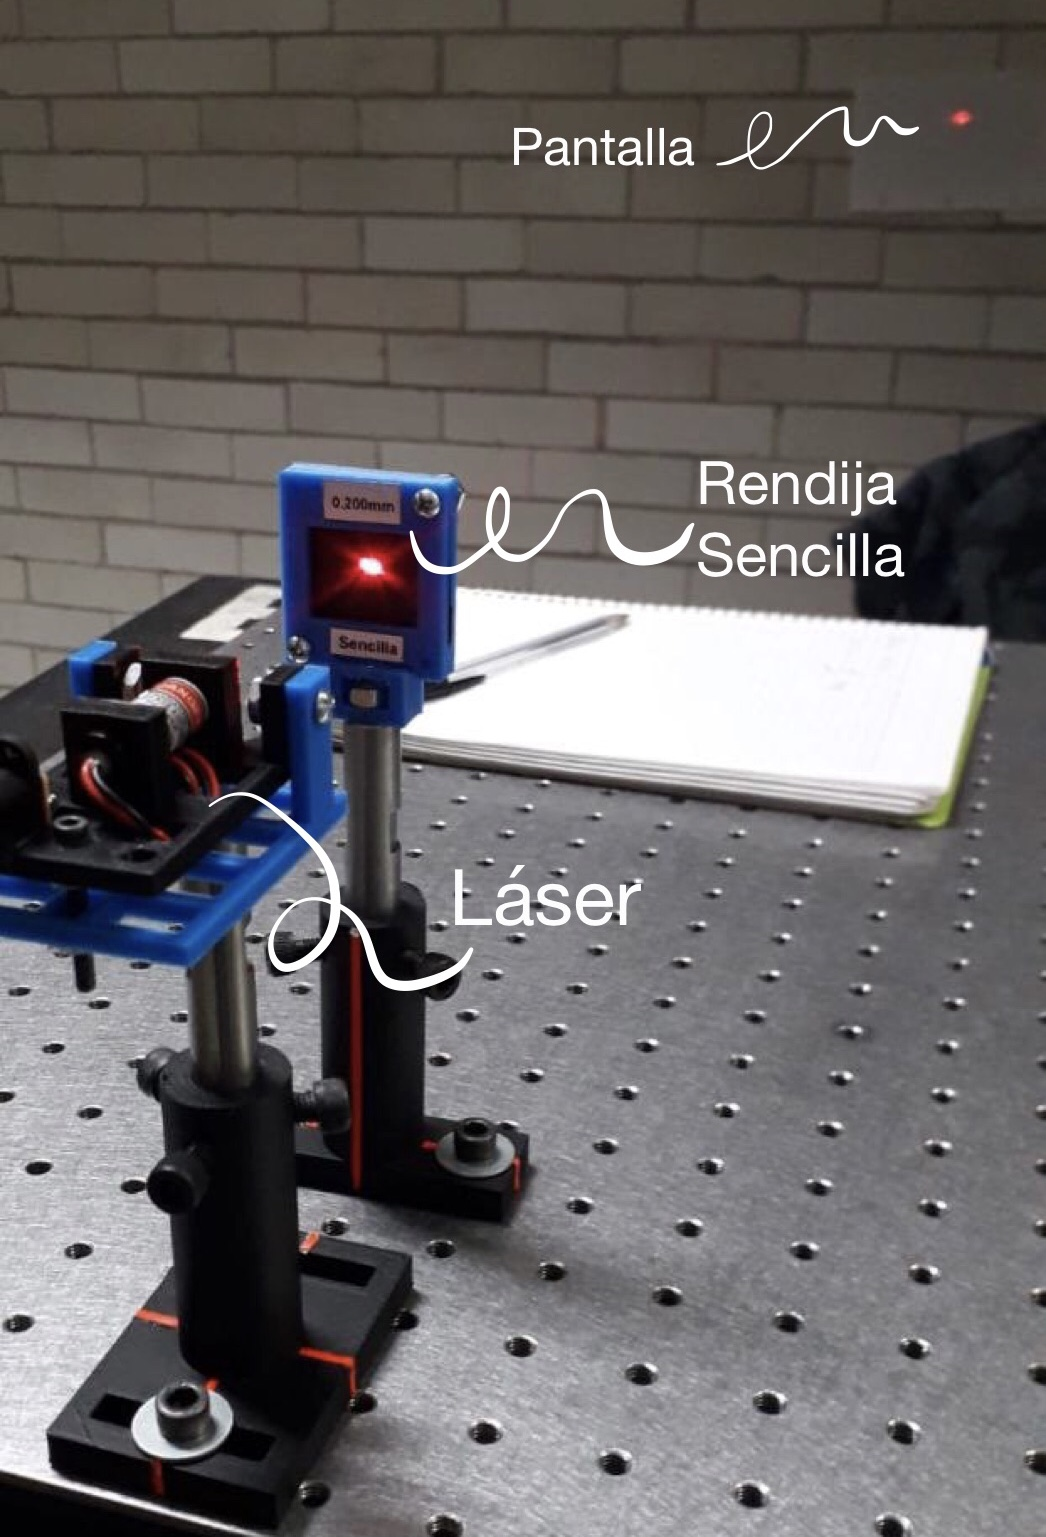
\includegraphics[width=0.17\textwidth]{Desarrollo experimental/97B94466-881A-4F6D-A677-D17587296DC4.jpeg}}
  \subfloat[Franjas de interferencia vistas en el experimento]{
   \label{f:tigre}
    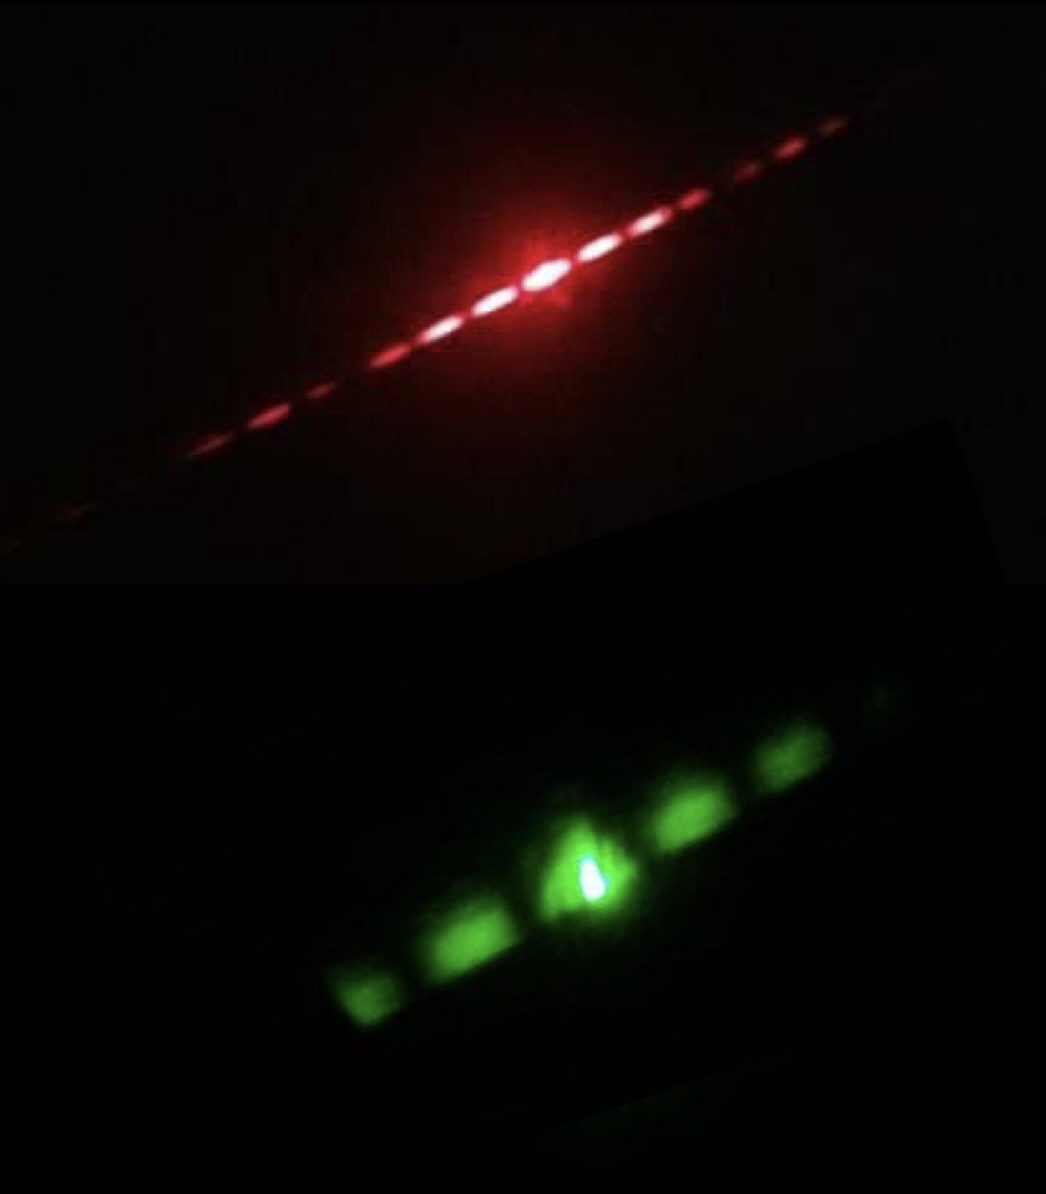
\includegraphics[width=0.20\textwidth]{Desarrollo experimental/8A6A217C-CC85-4BC9-985D-D1D73428542B.jpeg}}
 \caption{\textbf{Experimento de Young.} En la figura 3(a) se observa el arreglo experimental utilizado para observar lo patrones de interferencia de una doble rendija. En la figura 3(b) se observan los patrones de interferencia vistos para el láser rojo y verde. }
 \label{f:animales}
\end{figure}
\section*{\textcolor{carmine}{Resultados y Análisis.}}

\subsection*{\textcolor{carmine}{Interferencia}}

Despejando $a$ de la ecuación (1) y propagando su incertidumbre se tiene,

\begin{equation*}
    a = \frac{\lambda L}{y_{\text{min}}} \left(m \pm \frac{1}{2}\right)
\end{equation*}



\begin{equation*}
    \Delta a = \sqrt{ \left(\frac{\partial a}{\partial y_{\text{min}}}\Delta y_{\text{min}}\right)^{2} + \left(\frac{\partial a}{\partial L} \Delta L\right)^{2}}= \frac{\lambda L}{y_{\text{min}}}\sqrt{\left(\frac{\Delta y_{\text{min}}}{y_{\text{min}}}\right)^{2} + \left(\frac{\Delta L}{L}\right)^{2}}
\end{equation*}

Las separaciones entre las rendijas $a$ obtenidas son las siguientes:

\begin{figure}[H]
    \centering
    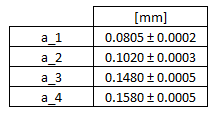
\includegraphics{tablas/tabla 1.PNG}
    \caption{Tabla de distancias entre rendijas $a$.}
    \label{fig:my_label}
\end{figure}

ahora despejando $\lambda$ de la ecuación (1) y propagando su incertidumbre se obtiene la relación,

\begin{equation*}
    \lambda_i = \frac{a_i y_{\text{min}}}{L (m \pm \frac{1}{2})}
\end{equation*}


\begin{equation*}
    \Delta \lambda_i = \sqrt{ \left(\frac{\partial \lambda_i}{\partial y_{\text{min}}}\Delta y_{\text{min}}\right)^{2} + \left(\frac{\partial \lambda_i}{\partial L} \Delta L\right)^{2} + \left(\frac{\partial \lambda_i}{\partial  a_i} \Delta a_i\right)^{2}}= \frac{a_i y_{\text{min}}}{L (m \pm \frac{1}{2})} \sqrt{\left(\frac{\Delta y_{\text{min}}}{y_{\text{min}}}\right)^{2}+ \left(\frac{\Delta L}{L}\right)^{2} +\left(\frac{\Delta a_i}{a_i}\right)^{2}}
\end{equation*}

Las longitudes de onda $\lambda$ obtenidas son las siguientes:


\begin{figure}[H]
    \centering
    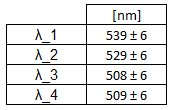
\includegraphics{tablas/tabla 2.PNG}
    \caption{Tabla de longitudes de onda para el láser verde.}
    \label{fig:my_label}
\end{figure}


El promedio de las longitudes de onda nos da un valor para el láser verde de:


\begin{equation*}
    \lambda_{\text{verde}} = (521 \pm 6) \text{ nm}
\end{equation*}




\subsection*{\textcolor{carmine}{Difracción}}

Despejando $b$ de la ecuación (2) y propagando su incertidumbre se tiene,

\begin{equation*}
    b = \frac{m \lambda L}{y_{\text{min}}}
\end{equation*}



\begin{equation*}
    \Delta b =\frac{m \lambda L}{y_{\text{min}}} \sqrt{\left(\frac{\Delta y_{\text{min}}}{y_{\text{min}}}\right)^{2} + \left(\frac{\Delta L}{L}\right)^{2}}
\end{equation*}

Los anchos de las rendijas simples $b$  son:

\begin{figure}[H]
    \centering
    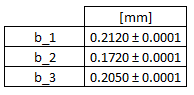
\includegraphics{tablas/tabla 3.PNG}
    \caption{Tabla de anchos de las rendijas simples.}
    \label{fig:my_label}
\end{figure}

Despejando $\lambda$ de la ecuación (2) y propagando su incertidumbre se tiene,

\begin{equation*}
    \lambda_i = \frac{b_i y_{\text{min}}}{mL}
\end{equation*}

\begin{equation*}
    \Delta \lambda_i = \frac{b_i y_{\text{min}}}{mL} \sqrt{\left(\frac{\Delta y_{\text{min}}}{y_{\text{min}}}\right)^{2} + \left(\frac{\Delta L}{L}\right)^{2} + \left(\frac{\Delta b_i}{b_i}\right)^{2}}
\end{equation*}

Las longitudes de onda $\lambda$ son:

\begin{figure}[H]
    \centering
    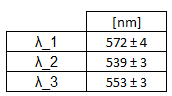
\includegraphics{tablas/tabla 4.PNG}
    \caption{Tabla de longitudes de onda para el láser verde.}
    \label{fig:my_label}
\end{figure}

El promedio de las longitudes de onda nos da un valor para el láser verde de:

\begin{equation*}
    \lambda_{\text{verde}} = (555 \pm 3) \text{ nm}
\end{equation*}

\section*{\textcolor{carmine}{Discusión y Conclusión.}}
Se obtuvo que la primer distancia entre rendijas era de 
$$(0.0805\hspace{0.1cm}\pm\hspace{0.1cm}0.0002)\hspace{0.1cm}\text{ mm}$$
Para la segunda se tiene un valor de: $$(0.1020\hspace{0.1cm}\pm\hspace{0.1cm}0.0001)\hspace{0.1cm}\text{ mm}$$ 
Para la tercer rendija el valor fue de $$(0.1480\hspace{0.1cm}\pm\hspace{0.1cm}0.0001)\hspace{0.1cm}\text{ mm}$$ 
Para la última rendija se obtuvo un valor de $$(0.1580\hspace{0.1cm}\pm\hspace{0.1cm}0.0001)\hspace{0.1cm}\text{ mm}$$ 
Se obtuvo una longitud de onda del láser verde de:
$$\lambda_{\text{verde}} = (521 \pm 6) \text{ nm}$$ 
Por otro lado, con rendijas sencillas se obtuvo que el ancho de la primer rendija era de $$(0.2120\hspace{0.1cm}\pm\hspace{0.1cm}0.0001)\hspace{0.1cm}\text{ mm}$$ 
Para la segunda rendija se obtuvo un valor de  $$(0.1720\hspace{0.1cm}\pm\hspace{0.1cm}0.0001)\hspace{0.1cm}\text{ mm }$$ 
Para la última rendija se obtuvo: $$(0.2050\hspace{0.1cm}\pm\hspace{0.1cm}0.0001)\hspace{0.1cm}\text{ mm }$$
Se obtuvo una longitud de onda del láser verde de:
$$\lambda_{\text{verde}} = (555 \pm 3) \text{ nm}$$
Comparando con los valores esperados presentados en la introducción vemos que se obtuvieron valores similares, podemos decir que el experimento se realizó de manera exitosa, por los instrumentos de medición utilizados se obtuvieron datos precisos y un poco exactos.

\nocite{*}

\bibliography{biblio}

\end{document}